\documentclass[10pt,conference]{IEEEtran}
\IEEEoverridecommandlockouts
% The preceding line is only needed to identify funding in the first footnote. If that is unneeded, please comment it out.
\usepackage{balance}
\usepackage{xspace}
\usepackage{graphicx}
\usepackage[mathscr]{euscript}
\usepackage{listings}
\usepackage{enumitem}
\usepackage{multirow}
\usepackage{amsmath,amssymb}
\usepackage[usenames, dvipsnames]{color}
\usepackage{wrapfig}
\usepackage{cite}
\usepackage{float}
\usepackage[flushleft]{threeparttable}
\usepackage{pifont}
\usepackage{scrextend}
\usepackage{soul}
\usepackage{color} 
\usepackage{fancyvrb}
\usepackage{hyperref}
\usepackage{lettrine}


\def\BibTeX{{\rm B\kern-.05em{\sc i\kern-.025em b}\kern-.08em
    T\kern-.1667em\lower.7ex\hbox{E}\kern-.125emX}}
\begin{document}

\title{Preconditions on Rename Refactorings}

\author{
\IEEEauthorblockN{Soumya Mudiyappa}
\IEEEauthorblockA{\textit{West Chester University}\\fs926226@wcupa.edu}
\and
\IEEEauthorblockN{Swetchha Shukla}
\IEEEauthorblockA{\textit{West Chester University}\\ss928947@wcupa.edu}
\and
\IEEEauthorblockN{Yung-Chen Cheng}
\IEEEauthorblockA{\textit{West Chester University}\\yc917559@wcupa.edu}
}

\maketitle

\section{\textbf{Rename Refactorings}}
\lettrine{R} {ename} Refactoring changes the name of identifiers in a program without changing the program's behavior.
There are five types of Rename Refactoring in Java: 
\begin{enumerate}
	\item Rename Class Declarations 
	\item Rename Method Declarations  
	\item Rename Field Declarations  
	\item Rename Local Variables  
	\item Rename Package Declarations
\end{enumerate}

\section{\textbf{Preconditions of Rename Class Refactoring}}
Rename Class Refactoring (RcR) changes the name of the class and all references to that class to the new name without changing its behavior. There are certain preconditions required for RcR. 
\begin{enumerate}
	\item The target class cannot be duplicate with any existing class within same package after rename.
	\item The target class cannot be duplicate with any imported class from different package after rename.
	\item The target class file name cannot be duplicate with any existing java file name within same package after rename.
\end{enumerate}

\subsection{The target class cannot be duplicate with any existing class within same package after rename.}

When we try to rename a class with any existing class name, the Java compiler produces syntax error \textit{``Please choose another name"}.~\cite{EclipseWebPage} The classes will be conflicted if we rename refactor the target class using the name of an existing class in the same package. So, we can not have duplicate class names in the same package. 

For example, if we want to rename refactor the class name from \textsl{A} to \textsl{B} as in Fig. \ref{fig:afterrr}, then the Java compiler produces an error that B.java already exists as shown in Fig. \ref{fig:renameclassname}.

\begin{figure}[th]
\centering
\begin{minipage}[t]{0.45\linewidth}
\begin{lstlisting}[language=java, basicstyle=\scriptsize\ttfamily,frame=single]
package p;

class A{
}
	
class B{
}

class C{
}
 
\end{lstlisting}
\centering{(a) Before}
\end{minipage}
\hfill
\begin{minipage}[t]{0.45\linewidth}
\begin{lstlisting}[language=java, basicstyle=\scriptsize\ttfamily,frame=single]
package p;

class B{
}	

class B{
}

class C{
}

\end{lstlisting}
\centering{(b) After}
\end{minipage}
\caption{\textbf{Example of RcR from A to B}}
\label{fig:afterrr}
\end{figure}

\begin{figure}[H]
\centerline{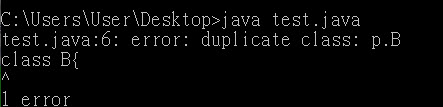
\includegraphics[width=85mm,scale=0.5]{SCN.jpg}}
\caption{\textbf{Compile error for using same class name after RcR}}
\label{fig:renameclassname}
\end{figure}

Also, this precondition is applicable even if the classes are defined in separate java files or any file is empty but are within the same folder. In Fig. \ref{fig:empty}, we try to apply RcR from \emph{A to C} or \emph{B to C} where C.java is an empty file, the compiler produces an error as shown in Fig. \ref{fig:efr}. 

\begin{figure}[th]
\centering
\begin{minipage}[t]{0.45\linewidth}
\begin{lstlisting}[language=java, basicstyle=\scriptsize\ttfamily,frame=single]
A.java

public class A{
}
	
class B{
}


C.java
//empty file
 
\end{lstlisting}
\centering(a) Before
\end{minipage}
\hfill
\begin{minipage}[t]{0.45\linewidth}
\begin{lstlisting}[language=java, basicstyle=\scriptsize\ttfamily,frame=single]
A.java

public class A{
}
	
class C{
}


C.java
//empty file

\end{lstlisting}
\centering(b) After
\end{minipage}
\caption{\textbf{RcR from B to C even if C.java is empty}}
\label{fig:empty}
\end{figure}

\begin{figure}[H]
\centerline{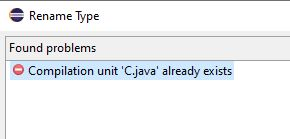
\includegraphics[width=85mm,scale=0.5]{EFE.jpg}}
\caption{\textbf{Compile error for same file name after RcR}}
\label{fig:efr}
\end{figure}


Furthermore, this precondition is also applicable to nested classes. The examples below show that for RcR we can not use the same name either as inner or as outer class for nested classes like Fig. \ref{fig:original}.

\begin{figure}[th]
\centering
\begin{minipage}[t]{0.5\linewidth}
\begin{lstlisting}[language=java, basicstyle=\scriptsize\ttfamily,frame=single]
package p;

public class A{	

  class M{
  }

  class N{
  }
} 
\end{lstlisting}
\end{minipage}
\caption{\textbf{Nested Class before RcR}}
\label{fig:original}
\end{figure}

\textbf{Example 1:} In order to implement RcR for inner class, we should pre-check that we do not use the same name as any of other inner class name. From Fig. \ref{fig:nestedclass1}, when we try to rename refactor the inner class from M to N, the Java compiler produces an error as shown in Fig. \ref{fig:NC1}.

\begin{figure}[th]
\centering
\begin{minipage}[t]{0.5\linewidth}
\begin{lstlisting}[language=java, basicstyle=\scriptsize\ttfamily,frame=single]
package p;

public class A{	
    
  class N{
  }
    
  class N{
  }
} 
\end{lstlisting}
\end{minipage}
\caption{\textbf{Example 1 for Nested Class after RcR from M to N}}
\label{fig:nestedclass1}
\end{figure}

\begin{figure}[H]
\centerline{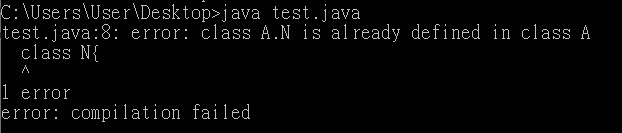
\includegraphics[width=75mm,scale=0.4]{NC1.jpg}}
\caption{\textbf{Compile error for duplicate inner class name after RcR}}
\label{fig:NC1}
\end{figure}

\textbf{Example 2:} In order to implement RcR for outer class, we should pre-check that we do not use the same name as any of the inner class name and vice-versa. From Fig. \ref{fig:nestedclass2}, when we try to use same name for outer class and inner class, the Java compiler produces an error as shown in Fig. \ref{fig:NC2} and Fig. \ref{fig:NC3}.

\begin{figure}[th]
\centering
\begin{minipage}[t]{0.45\linewidth}
\begin{lstlisting}[language=java, basicstyle=\scriptsize\ttfamily,frame=single]
package p;

public class M{	
  
  class M{
  }
	
  class N{
  }
} 
\end{lstlisting}
\centering{(a) After RcR on Outer Class A to M}
\end{minipage}
\hfill
\begin{minipage}[t]{0.45\linewidth}
\begin{lstlisting}[language=java, basicstyle=\scriptsize\ttfamily,frame=single]
package p;

public class A{	
    
  class A{
  }
    
  class N{
  }
} 
\end{lstlisting}
\centering{(b) After RcR on Inner Class N to A}
\end{minipage}
\caption{\textbf{Example 2 of Nested Class after RcR}}
\label{fig:nestedclass2}
\end{figure}

\begin{figure}[H]
\centerline{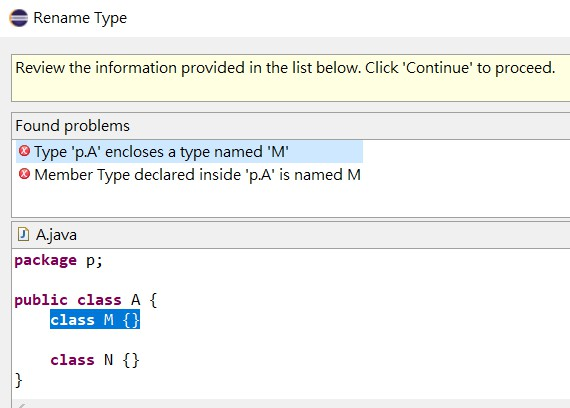
\includegraphics[width=75mm,scale=0.4]{NC2.jpg}}
\caption{\textbf{Compile error for RcR outer class same as inner class name}}
\label{fig:NC2}
\end{figure}

\begin{figure}[H]
\centerline{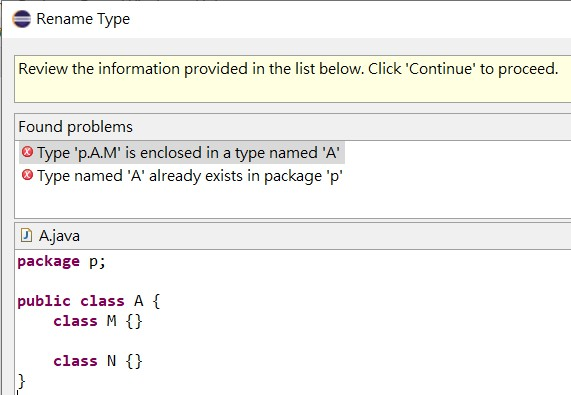
\includegraphics[width=75mm,scale=0.4]{NC3.jpg}}
\caption{\textbf{Compile error for RcR inner class same as outer class name}}
\label{fig:NC3}
\end{figure}

Therefore, checking whether a class with the same name already exists in a package should be the first precondition for RcR. 
   
\label{sec:precon1}
	
\subsection{The target class cannot be duplicate with any imported class from different package after rename.}

If a class is imported from different package, we have to pre-check that the new name of the target class is not duplicate with the imported class after rename refactoring. 

\begin{figure}[th]
\centering
\begin{minipage}[t]{0.4\linewidth}
\begin{lstlisting}[language=java, basicstyle=\scriptsize\ttfamily,frame=single]
package q;
import p.C;

class A{
}

class B{
} 
\end{lstlisting}
\centering(a) Before
\end{minipage}
\hfill
\begin{minipage}[t]{0.4\linewidth}
\begin{lstlisting}[language=java, basicstyle=\scriptsize\ttfamily,frame=single]
package q;
import p.C;

class A{
}

class C{
} 
\end{lstlisting}
\centering(b) After
\end{minipage}
\caption{\textbf{RcR from B to C}}
\label{figure:fig2}
\end{figure}

In Fig. \ref{figure:fig2} (a), we see that class B is not duplicate with class A and we can implement RcR on class B to any other name except `A' as mentioned in section \ref{sec:precon1}. However, in Fig. \ref{figure:fig2} (b), when we try to implement RcR from \emph{B to C}, Java compiler produces an error \textit{``a compilation unit must not import and declare a type with the same name''}~\cite{EclipseWebPage} as shown in Fig. \ref{figure:comperr}. This is because the compiler cannot distinguish between the \emph{imported class C} of package `p' and the \emph{existing class C} of package `q'. 

\begin{figure}[H]
\centerline{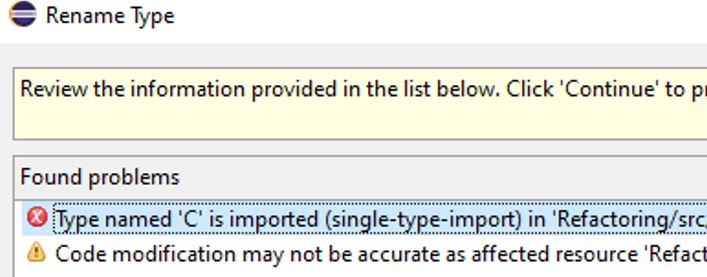
\includegraphics[width=85mm,scale=0.5]{CUE.jpg}}
\caption{\textbf{Compilation Unit Error} }
\label{figure:comperr}
\end{figure}

Therefore, it is essential to pre-check that the target class should not have duplicate name with any of imported class after RcR.
\label{sec:precon2}

\subsection{The target sub-class cannot be duplicate with any imported class into its parent class from another package.}

If we try renaming a subclass with the same name as the class imported into its parent class from another package, compiler produces the error as `a compilation unit must not import and declare a type with the same name'~\cite{EclipseWebPage}. 
To rename a class or subclass for refactoring the code, some of the necessary preconditions have to be checked. This precondition can be explained by the following example.

\begin{figure}[th]
\centering
\begin{minipage}[t]{0.45\linewidth}
\begin{lstlisting}[language=java, basicstyle=\scriptsize\ttfamily,frame=single]	
package q;
import p.C;
class A{	
}
class B extends A{	
}	
\end{lstlisting}
\tiny{(a) Before renaming Subclass B}
\end{minipage}
\hfill
\begin{minipage}[t]{0.45\linewidth}
\begin{lstlisting}[language=java, basicstyle=\scriptsize\ttfamily,frame=single]
package q;
import p.C;
class A{	
}
class C extends A{	
}	
\end{lstlisting}
\tiny{(b) After Renaming Subclass B to C}
\end{minipage}
\caption{Precondition for Renaming Sub-class}
\label{figure:fig7}
\end{figure}

From the above figure \ref{figure:fig7}, We see that if one has imported class C from  package  p to the parent Class A and if we try to rename the sub-class B to C, Compiler produces  the error as given in the figure \ref{figure:fig8} . As mentioned in  section \ref{sec:precon2}, the same precondition also holds good for renaming a sub-class. Before renaming the sub-class, one has to check the precondition that the  target sub-class cannot be duplicate with any imported class into its parent class from another package.

\begin{figure}[htbp]
\centerline{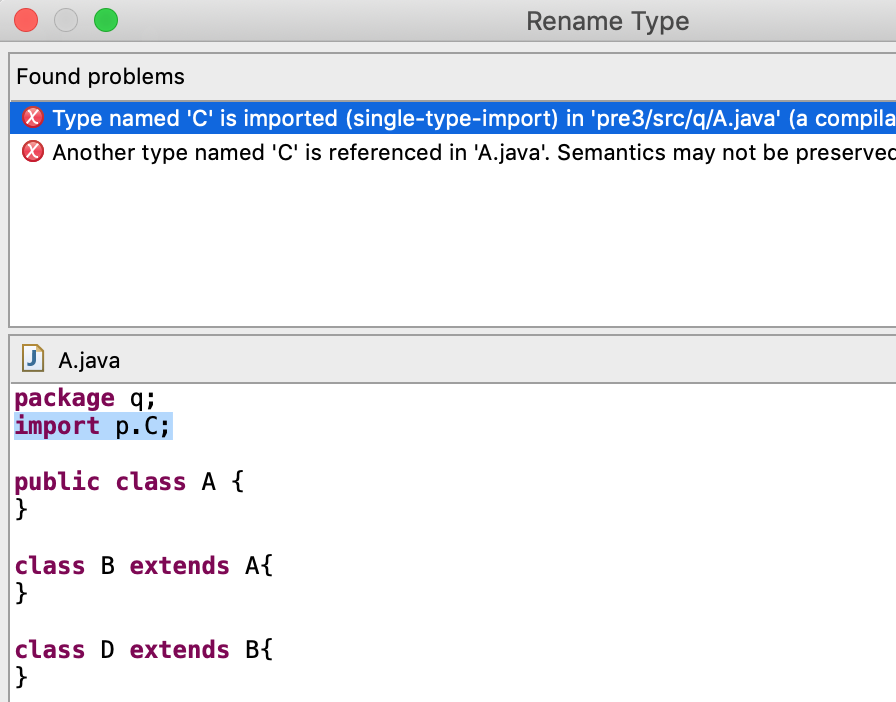
\includegraphics[width=85mm,scale=0.5]{precond3.png}}
\caption{Error produced after renaming the sub-class.}
\label{figure:fig8}
\end{figure}
\label{sec:precon3}

\section{\textbf{Preconditions of Rename Method Refactoring}}

\section{\textbf{Preconditions of Rename Field Refactoring}}
Fields are the variables of a class i.e. instance variables and static variables.

Rename Field Refactoring (RfR) changes the declaration and references to the field variables to the new name without changing its behavior.
There are certain preconditions required for RfR.

\begin{enumerate}
	\item The target name of field variable cannot be duplicate with any existing field within same class after rename.
	\item The target name of field variable cannot be duplicate with any local variable within same method after rename.
	\item The duplicate field variable in a child class cannot reduce visibility. 
\end{enumerate}

\subsection{The target name of field cannot be duplicate with any existing field within same class after rename.}

In order to apply RfR we have to pre-check that the new name of the field is not duplicate with any existing field name of any data type within same class. From Fig. \ref{figure:field}(a), when we apply RfR from \emph{`j' to `i'} as shown in Fig. \ref{figure:field}(b), Java compiler produces an error \textit{``variable i is already defined in class A''}. This is because of the conflict for duplicate names for field variables. Similarly when we apply RfR from \emph{`s' to `i'} as shown in Fig. \ref{figure:field}(c), Java compiler produces an error \textit{``variable i is already defined in class A''}. 

\begin{figure}[th]
\centering	
\begin{minipage}[t]{0.45\linewidth}
\begin{lstlisting}[language=java, basicstyle=\scriptsize\ttfamily,frame=single]
class A {

   int i = 0;
   int j = 2;
   String s = "hi";
}

\end{lstlisting}
\centering(a) Before
\end{minipage}
\hfill
\begin{minipage}[t]{0.45\linewidth}
\begin{lstlisting}[language=java, basicstyle=\scriptsize\ttfamily,frame=single]
class A {

   int i = 0;
   int i = 2;
   String s = "hi";
}
\end{lstlisting}
\centering(b) After Rename Refactoring Field j to i
\end{minipage}

\centering
\begin{minipage}[t]{0.45\linewidth}
\begin{lstlisting}[language=java, basicstyle=\scriptsize\ttfamily,frame=single]
class A {

   int i = 0;
   int j = 2;
   String i = "hi";
}
\end{lstlisting}
\centering(c) After Rename Refactoring Field s to i
\end{minipage}
\caption{\textbf{Rename Refactoring on field variables}}
\label{figure:field}
\end{figure}


\subsection{The target name of field cannot be duplicate with any local variable within same method after rename.}
In order to apply RfR we have to pre-check that the new name of field is not duplicate with any local variable name, if field is being used in the same block as local variable. 

As shown in Fig. \ref{figure:sameBlock}(a), the output is `0'. However, after we apply RfR from $x$ to $y$ as shown in Fig. \ref{figure:sameBlock}(b), the output is `1'. Although the Java compiler do not produce any error but the behavior of code has changed since the output after RfR has changed. This is because if a field variable and a local variable have the same name, then the local variable will be accessed. This process effectively shadows the field variable and therefore known as \textit{Variable Shadowing}. Therefore, it is essential to pre-check that the new name of field is not duplicate with any existing local variable if both are used in same block.
 

\begin{figure}[th]
\centering
\begin{minipage}[t]{0.47\linewidth}
\begin{lstlisting}[language=java, basicstyle=\scriptsize\ttfamily,frame=single]
class A{

   int x = 0;
	
   void m(int y) {
	
      //Output: 0
      System.out.print(x);
   }
	
   void main(String[] args) {
	
      this.m(1);
   }
}

\end{lstlisting}
\centering(a) Before
\end{minipage}
\hfill
\begin{minipage}[t]{0.47\linewidth}
\begin{lstlisting}[language=java, basicstyle=\scriptsize\ttfamily,frame=single]
class A{

   int y = 0;
	
   void m(int y) {
	
      //Output: 1
      System.out.print(y);
   }
	
   void main(String[] args) {

      this.m(1);
   }
}
\end{lstlisting}
\centering(b) After
\end{minipage}
\caption{\textbf{Rename Refactoring Field x to y}}
\label{figure:sameBlock}
\end{figure}

The same concept is applied to class hierarchies. A field variable declared within a parent class will be shadowed by any variable with the same name in a child class. As shown in Fig. \ref{figure:classEx}(a), the output is `0'. However, after we apply RfR on field variable of a child class from $j$ to $i$ as shown in Fig. \ref{figure:classEx}(b), the output is `1'. This Variable Shadowing has changed the original behavior of the program after RfR. 

\begin{figure}[th]
\centering
\begin{minipage}[t]{0.47\linewidth}
\begin{lstlisting}[language=java, basicstyle=\scriptsize\ttfamily,frame=single]
class A {

   int i = 0;
   
   void main(String[] args) {

      B b = new B();
	      
      // Output: 0
      System.out.print(b.i); 
   }
}

class B extends A {

   int j = 1; 
}
\end{lstlisting}
\centering{(a) Before}
\end{minipage}
\hfill
\begin{minipage}[t]{0.47\linewidth}
\begin{lstlisting}[language=java, basicstyle=\scriptsize\ttfamily,frame=single]
class A {

   int i = 0;
   
   void main(String[] args) {

      B b = new B();
	      
      // Output: 1
      System.out.print(b.i); 
   }
}

class B extends A {

   int i = 1; 
}
\end{lstlisting}
\centering{(b) After }
\end{minipage}
\caption{\textbf{Rename Refactoring on child class field variable j to i}}
\label{figure:classEx}
\end{figure}

Therefore, it is essential to pre-check that the duplicate field variables in parent and child class does not result in variable shadowing. 

\subsection{The duplicate field variable in a child class cannot reduce visibility.}

The child class variables are able to reduce the visibility of the parent class variables. The use of access modifiers helps with visible duplicate field variables, however there is a proper hierarchy for access modifiers to be followed for duplicate variables.


\begin{center}
\textbf{public $>$ protected $>$ package-public $>$ private}
\end{center}


\begin{figure}[th]
\centering
\begin{minipage}[t]{0.47\linewidth}
\begin{lstlisting}[language=java, basicstyle=\scriptsize\ttfamily,frame=single]
class A {

   public int i = 0;
	
   void main(String[] args) {
	
      B b = new B();
      
      // Output: 0
      System.out.print(b.i); 
   }
}

class B extends A {

   private int j = 1;
}
\end{lstlisting}
\centering{(a) Before}
\end{minipage}
\hfill
\begin{minipage}[t]{0.47\linewidth}
\begin{lstlisting}[language=java, basicstyle=\scriptsize\ttfamily,frame=single]
class A {

   public int i = 0;
	
   void main(String[] args) {
	
      B b = new B();
      
      // Error
      System.out.print(b.i); 
   }
}

class B extends A {

   private int i = 1;
}
\end{lstlisting}
\centering{(b) After}
\end{minipage}
\caption{\textbf{Rename Refactoring on child class field j to i}}
\label{figure:jtoi}
\end{figure}


As shown in Fig. \ref{figure:jtoi}(a), the two field variables $i$ and $j$ are completely distinct and have completely separate visibilities in different classes. However, on applying RfR on child class variable from $j$ to $i$ as shown in Fig. \ref{figure:jtoi}(b), the public visibility of field variable $i$ gets reduced to private and Java compiler produces an error \textit{``field B.i is not visible''}. 

Therefore, it is essential to pre-check that the new name of the field variable does not result in visibility reduction.  

\section{\textbf{Preconditions of Rename Local Variable Refactoring}}
A local variable is a variable declared inside a method and it is only accessible inside the method that declared it

Rename Local Variable Refactoring (RvR) changes the name of the local variable and all references to that variable to the new name without changing its behavior. There are certain preconditions required for RvR.
\begin{enumerate}
\item The renamed local variable cannot be duplicate with any of the existing local variable in a method or block or constructor.
\item The renamed local variable must not result in variable shadowing.
\end{enumerate}

\subsection{The renamed local variable cannot be duplicate with any of the existing local variable in a method.}
 
From Fig. \ref{figure:precond5_1} and Fig. \ref{figure:precond5_2}, we see two examples of duplicate local variable. In Example 1 when we apply RvR for local variable `x' to `num' , the java compiler produces the error as ``variable num is already defined in method m1(int)''. Similarly we cannot run RvR on  `y'  to `num' or `x'  to `y' . Renaming local variables to existing local variable in a method creates a conflict of duplicity in local variable.

Therefore, it is essential to pre-check that the target name of local variable should not have duplicate name with any of the existing local variable in a method after RvR.

\begin{figure}[th]
\centering
\begin{minipage}[t]{0.45\linewidth}
\begin{lstlisting}[language=java, basicstyle=\scriptsize\ttfamily,frame=single]
public class A {

    void m1(int num) {
       int x = 1; 
       int y = 2
    }
}
\end{lstlisting}
\centering(a) Before
\end{minipage}
\hfill
\begin{minipage}[t]{0.45\linewidth}
\begin{lstlisting}[language=java, basicstyle=\scriptsize\ttfamily,frame=single]
public class A {

    void m1(int num) {
        int num = 1; 
	int y = 2;
    }
}
\end{lstlisting}
\centering(b) After 
\end{minipage}
\caption{\textbf{Rename Refactoring Variable x to num}}
\label{figure:precond5_1}
\end{figure}

\begin{figure}[th]
\centering
\begin{minipage}[t]{0.45\linewidth}
\begin{lstlisting}[language=java, basicstyle=\scriptsize\ttfamily,frame=single]
public class A {

    void m1(int num) {
       int x = 1; 
       int y = 2
    }
}
\end{lstlisting}
\centering(a) Before 
\end{minipage}
\hfill
\begin{minipage}[t]{0.45\linewidth}
\begin{lstlisting}[language=java, basicstyle=\scriptsize\ttfamily,frame=single]
public class A {

    void m1(int num) {
        int y = 1; 
	int y = 2;
    }
}
\end{lstlisting}
\centering(b) After 
\end{minipage}
\caption{\textbf{Rename Refactoring Variable x to y}}
\label{figure:precond5_2}
\end{figure}

\subsection{The renamed local variable must not result in variable shadowing.}
Shadowing refers to the concept of using two variables with the same name within scopes that overlap. When we do that, the variable with the higher-level scope is hidden because the variable with lower-level scope overrides it. This results in the higher-level variable being ``shadowed''. 

\begin{figure}[th]
\centering
\begin{minipage}[t]{0.8\linewidth}
\begin{lstlisting}[language=java, basicstyle=\scriptsize\ttfamily,frame=single]
public class B {

    public int i = 2;
    
    public void display() {
      int j = 1;
      System.out.println(j); 		
   }

    public static void main(String args[]) {
    
      B b = new B();
      b.display();  //Outputs 1
   }
}
\end{lstlisting}
\centering(a) Before 
\end{minipage}
\hfill
\begin{minipage}[t]{0.8\linewidth}
\begin{lstlisting}[language=java, basicstyle=\scriptsize\ttfamily,frame=single]
public class B {

    public int i = 2;
    
    public void display() {
      int i = 1;
      System.out.println(i); 		
   }

    public static void main(String args[]) {
    
      B b = new B();
      b.display();  //Outputs 1
   }
}
\end{lstlisting}
\centering(b) After 
\end{minipage}
\caption{\textbf{Rename Refactoring Variable j to i }}
\label{figure:precond5_3}
\end{figure}


Suppose a local variable has the same name as one of the field variable(instance variable), the local variable shadows the field variable inside the method block. From Fig. \ref{figure:precond5_3}, when we access the variable in the method, the local variable value will be printed shadowing the field variable.

Similarly variable shadowing occurs when the same variables are defined in parent and child classes.
For Example, from Fig. \ref{figure:precond5_4}, after RvR from j to i and k to i ,when we try to access the variable `i' in methods through Class B and C, the respective local variable will be printed shadowing the field variable of its parent class.


\begin{figure}[th]
\centering
\begin{minipage}[t]{0.8\linewidth}
\begin{lstlisting}[language=java, basicstyle=\scriptsize\ttfamily,frame=single]
public class B {

    int i = 1;

    public void m1() {
      int j = 2;
      System.out.println(j);
   }
}

class C extends B {

    int k = 3;
}

public class Main {

    public static void main(String args[]) {
  
       B b = new B();
       b.m1();     // outputs 2
       C c = new C();
       c.m1();     // outputs 2

   }
}
\end{lstlisting}
\centering(b) Before 
\end{minipage}
\hfill
\begin{minipage}[t]{0.8\linewidth}
\begin{lstlisting}[language=java, basicstyle=\scriptsize\ttfamily,frame=single]
public class B {

    int i = 1;

    public void m1() {
      int i = 2;
      System.out.println(i);
   }
}

class C extends B {

    int i = 3;
}

public class Main {

    public static void main(String args[]) {
  
       B b = new B();
       b.m1();   // outputs 2
       C c = new C();
       c.m1();   // outputs 2
   }
}
\end{lstlisting}
\centering(b) After 
\end{minipage}
\caption{\textbf{Rename Refactoring Variables j to i  and k to i }}
\label{figure:precond5_4}
\end{figure}


Therefore, it is essential to pre-check that local variable must not result in variable shadowing after RvR.

\section{\textbf{Preconditions of Rename Package Refactoring}}
Rename Package Refactoring (RpR) changes the name of the package and all references to that package to the new name without changing its behavior. There is one precondition required for RpR.

For Rename Package Refactoring (RpR), we can not use duplicate package name within the same source folder. However, we can run RpR with same package name from different Java folders.

For example, we assume that there are two packages in one source folder as shown in Fig. \ref{fig:RpR}, we can not run RpR on package q to p since package p is already exist in the same source folder. 

\begin{figure}[th]
\centering
\begin{minipage}[t]{0.45\linewidth}
\begin{lstlisting}[language=java, basicstyle=\scriptsize\ttfamily,frame=single]
//A.java
package p;

class A{}
	
class B{}


//M.java
package q;

class M{}	

class N{}
\end{lstlisting}
\centering{(a) Before}
\end{minipage}
\hfill
\begin{minipage}[t]{0.45\linewidth}
\begin{lstlisting}[language=java, basicstyle=\scriptsize\ttfamily,frame=single]
//A.java
package p;

class A{}
	
class B{}


//M.java
package p;

class M{}	

class N{}


\end{lstlisting}
\centering{(b)After}
\end{minipage}
\caption{\textbf{Rename Refactoring Package q to p}}
\label{fig:RpR}
\end{figure}



%\bibliographystyle{IEEEtran}
%\bibliography{ref}

\end{document}
